% CHAPITRE 3
\chapter{Bilan de C de la tourbière de La Guette}
\newpage

\section{Introduction}

\section{Matériels et méthodes}

Distribution des embases aléatoire stratifiée

\subsection{méthodes de mesure}

\subsubsection{mesures de flux de gaz}
La mesure des flux de \coo et de \chh ont été effectué en utilisant la méthode décrite dans la partie~\ref{sec:clsd_chbr_method}.
Les mesures de \coo ont été effectué de mars 2013 à février 2015, avec une fréquence quasiment mensuelle (20 campagnes, pour 24 mois de mesure).

Les mesures de \chh ont été effectuées avec une fréquence moindre principalement liée au difficulté de mise en oeuvre de l'instrument SPIRIT (lourd, difficilement transportable dans un milieu tourbeux).

\subsubsection{Les facteurs contrôlants}

Les mesures manuelle effectuées sont la mesure de la pression atmosphérique, du PAR, des températures du sol à différentes profondeur, de la végétation.

Les mesures automatiquement acquise via une station météo campbell sont la température de l'air, température de la tourbe à X, X et X profondeur, vitesse et direction du vent, humidité relative de l'air, irradiation solaire, pression atmosphérique.

\subsection{modélisation du bilan de C}

\section{Évolution générale des facteurs contrôlants et des flux}

\subsection{Les facteurs contrôlants}

\begin{figure}
\centering
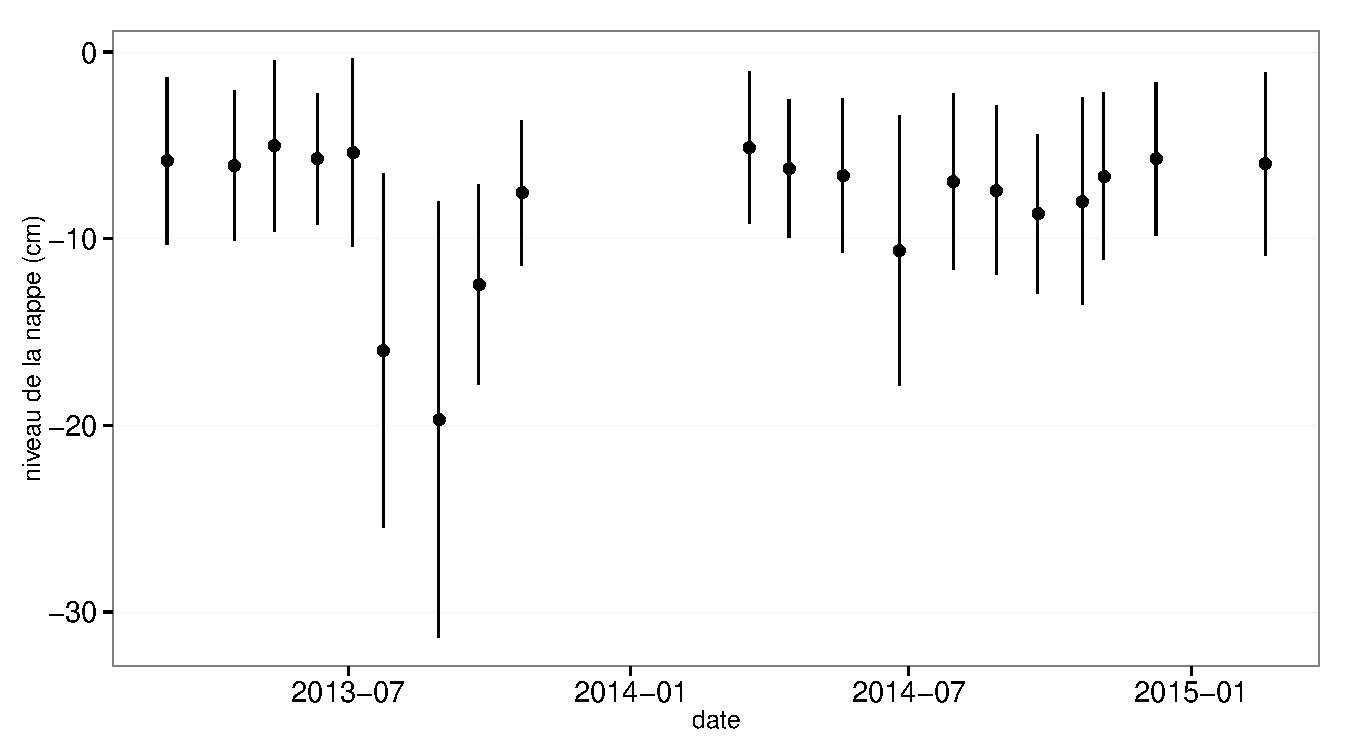
\includegraphics[width=\textwidth]{WTL_mean_evolution}
\caption{TODO}
\label{fig:WTL_mean_evolution}
\end{figure}

\subsection{Le \coo}

\subsubsection{PBB}

\begin{figure}
\centering
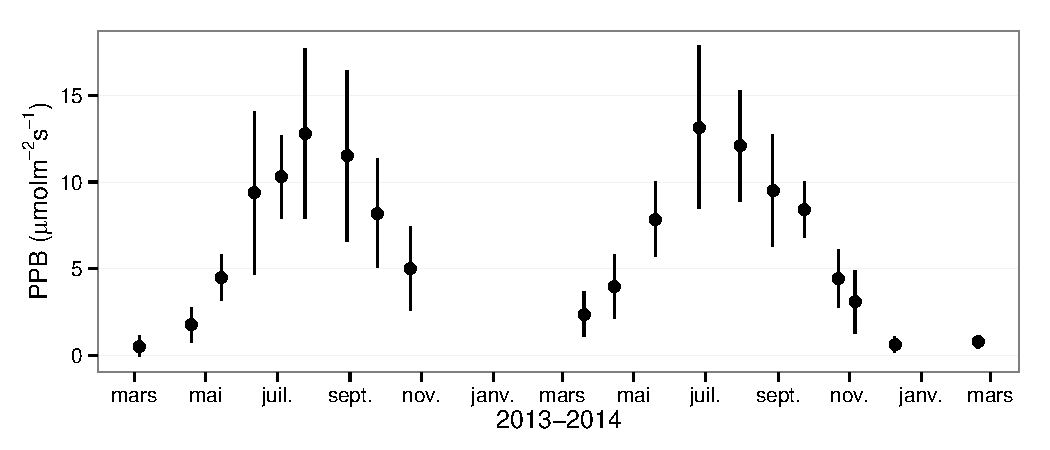
\includegraphics[width=\textwidth]{GPP_evolution_avg}
\caption{TODO}
\label{fig:GPP_evolution_avg}
\end{figure}

\subsubsection{ER}

\begin{figure}
\centering
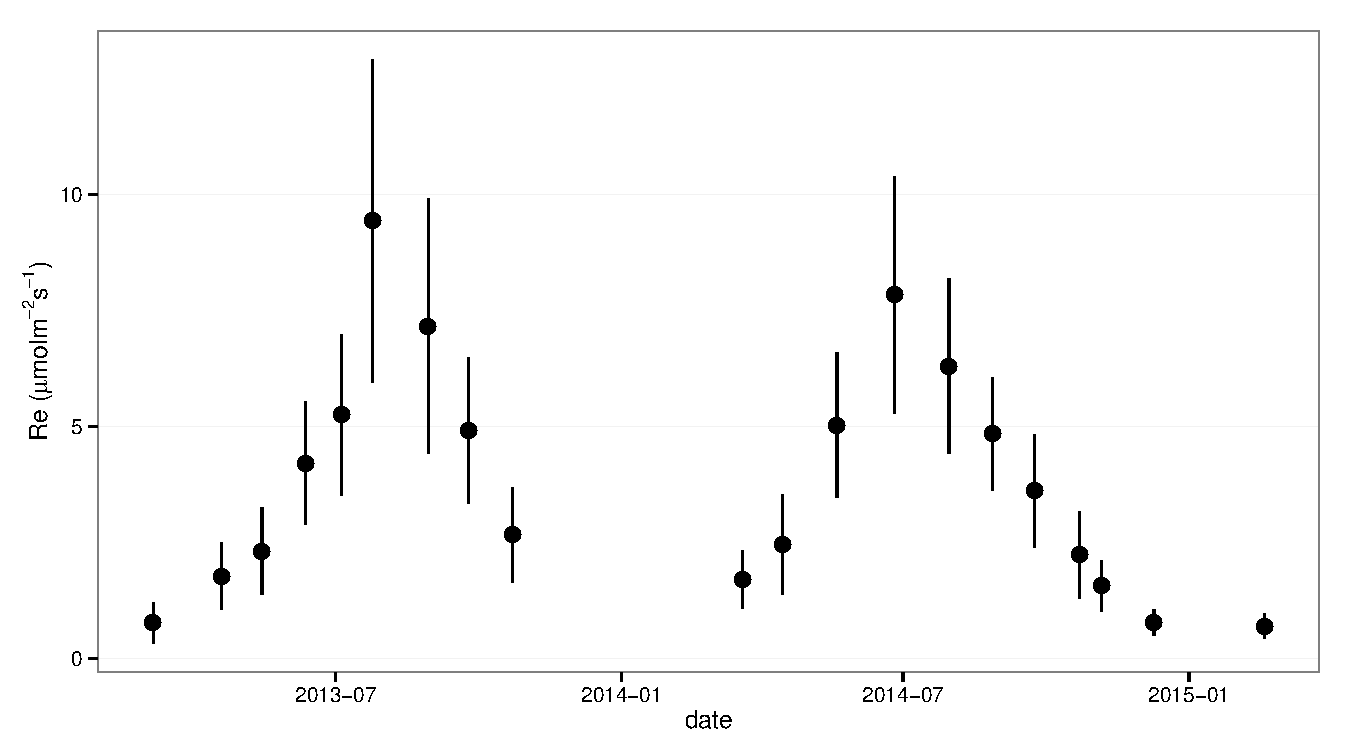
\includegraphics[width=\textwidth]{ER_evolution_avg}
\caption{TODO}
\label{fig:ER_evolution_avg}
\end{figure}

\subsubsection{ENE}

\begin{figure}
\centering
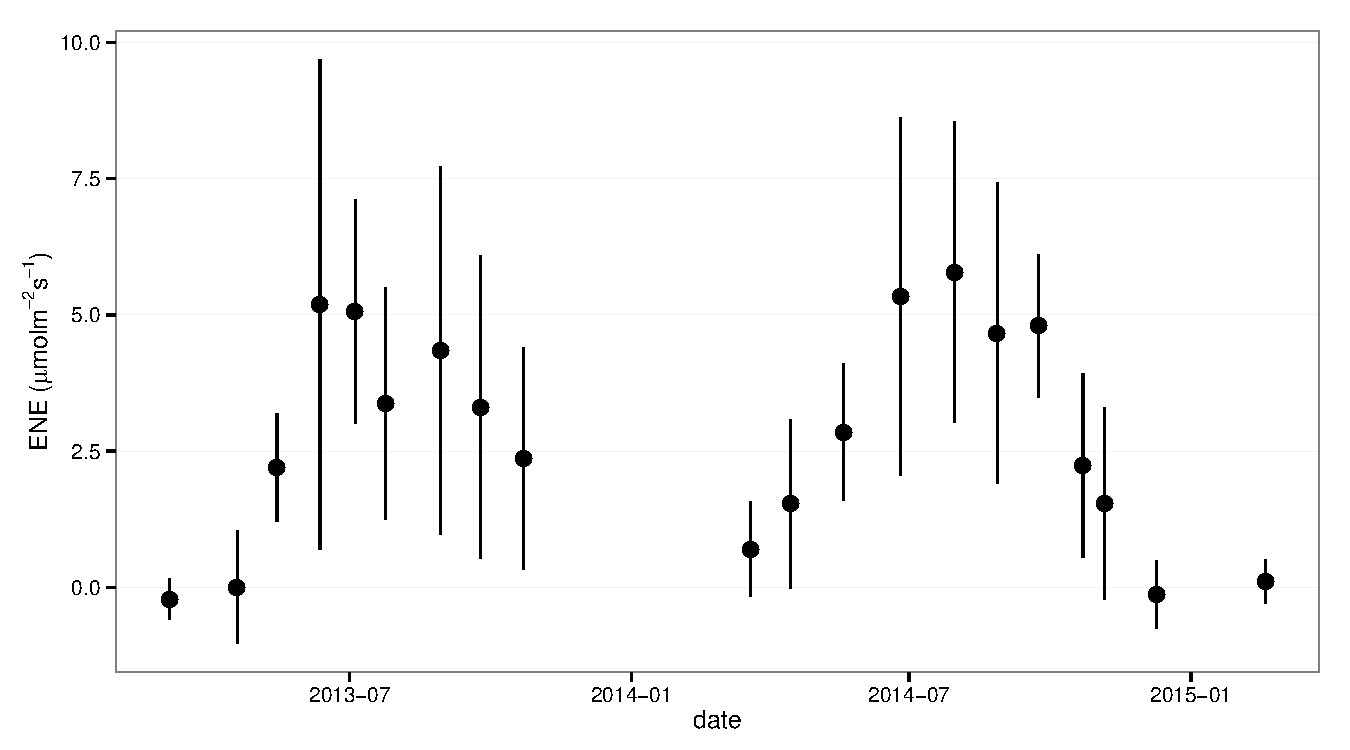
\includegraphics[width=\textwidth]{NEE_evolution_avg}
\caption{TODO}
\label{fig:NEE_evolution_avg}
\end{figure}

\subsection{Le \chh}
\subsection{Le Carbone Organique Dissous (COD)}

\section{Le bilan de carbone}

\section{Évaluation du bilan}

\subsection{sensibilité des paramètres}

\subsection{capacité à modéliser d'autres données}

\subsection{représentativité locale}

\section{représentativité locale ?}